\documentclass[10pt, conference, compsocconf]{IEEEtran}

\usepackage[pdftex]{graphicx}
\usepackage[cmex10]{amsmath}
\usepackage{url}
\usepackage{cite}

\begin{document}

\title{Estimating Driver's Required Attention Level via \\Flow-Based Processing of Dash Cam Videos}
\author{\IEEEauthorblockN{Corcoran Gary, Clark James}
\IEEEauthorblockA{Department of Electrical and Computer Engineering\\
McGill University\\
Montreal, Quebec\\
gary.corcoran@mail.mcgill.ca, clark@cim.mcgill.ca}
}

\maketitle

\begin{abstract}
The problem addressed in this paper is to estimate the driver's perceived attention levels from in-car dash cam videos via flow-based processing. The input data consists of in-car dash cam videos coupled with a simple optical flow-based calculation between sampled pairs of frames. The overall model is built upon Convolutional Neural Networks (CNNs) and Recurrent Neural Networks (RNNs). The dataset used is a collection of 1750 dash cam videos annotated as positive and negative examples of car accidents collected by Chan et al. \cite{10.1007/978-3-319-54190-7_9}. Instead of using these binary accident categories, each video is newly annotated with a perceived attention level of the driver. The videos are collectively annotated among a group of subjects with the average score taken as the final attention label. The four categories of attention levels are as follows: low attention, medium attention, high attention, and very high attention. From these attention levels a deep neural network is used to estimate the driver's attentiveness in various situations. The complete system runs in real-time; approximately ten frames per second.
\end{abstract}

\begin{IEEEkeywords}
Deep Convolutional Neural Networks, Recurrent Neural Networks, Long-Short Term Memory Units, Driver's Attention, Dash Cam Videos, Active Safety Systems.
\end{IEEEkeywords}

\IEEEpeerreviewmaketitle

\section{Introduction}
Even for the most experienced drivers, driving any vehicle is a very difficult task. This difficulty can be shown by the high number of collisions in Canada alone. In 2015, there were 118,404 collisions that were either fatal or involved a personal injury \cite{TrafficReport}. In about 84\% of all accidents the cause was traced back to driver error \cite{CognitiveModel}. 

Although the majority of vehicles are currently equipped with passive safety systems, i.e. systems to help reduce the outcome of an accident, such as seat belts, airbags, etc., there are still a high number of serious accidents. Newer intelligent car models are becoming equipped with active safety systems that utilize an understanding of the vehicle's state to avoid and minimize the effects of a crash. Some of these systems include collision warning and adaptive cruise control. Furthermore, research into these active safety systems have expanded into applications that work with or for the driver. This new generation of driver-assistance systems go beyond automated control systems by attempting to work in combination with a driver. These advanced safety systems include predicting driver intent \cite{doi:10.1177/154193120404801905}, warning drivers of lane departures \cite{ROB:ROB10056}, etc.

Active systems have many benefits, however, they are difficult to implement as they require knowledge about the driver, the vehicle, or the environment.

To address this problem, we look into requiring knowledge about the driver's perceived attention levels. To do this, low-level flow fields from in-car dash cam videos are processed and a neural network is built to label the driver's required attention level into four categories: low attention, medium attention, high attention and very high attention.

In particular, the two components of our proposed system are as follows: 1) From input dash cam videos estimate the driver's perceived attention level in real-time, 2) When the perceived attention level of the driver reaches a category of high or very high provide an alert to the driver to help redirect their attention.

To build the system, simple flow fields are extracted from sampled pairs of frames captured by the in-car dash cam and are used as input into a Convolutional Neural Network (CNN). The CNN architecture used is an 18-layer Residual Network (ResNet) \cite{DBLP:journals/corr/HeZRS15}. The last classification layer of the ResNet is removed and the resultant high-level flow features are used for further processing. These high-level features are extracted from each pair of frames and are passed into a Recurrent Neural Network (RNN). The RNN model uses Long Short-Term Memory (LSTM) units as building blocks for the network \cite{Hochreiter:1997:LSM:1246443.1246450}. Since the proposed algorithm assigns a single attention level to the full video sequence, only the final hidden state of the RNN model is used. This last hidden state is then feed into a softmax classifier to produce the final output of the network, i.e. the driver's perceived attention level.

As unseen videos are passed through the network, the model breaks them into sequences of variable length. Each sequence is passed through the complete network and provided with a final attention label. If a given label is categorized as requiring high or very high attention, an alert is provided to the driver. The complete process runs in real time (ten frames per second) on a laptop GPU.

\section{Related Work}
With many new technologies becoming embedded into users' everyday life, drivers need to make sure they are paying adequate attention to their surroundings. To this end, there has been numerous works on modeling and monitoring driver's attentiveness. Many of this work attempts to directly correlate attention to another means of measurement such as drowsiness, head movements/position, or alertness \cite{10.1007/3-540-48222-9_8}, \cite{WU20081556}, \cite{639576}, \cite{s121216937}. Although these systems can provide a broad understanding of the driver's attention level, there are always situations where a single measurement is not enough. In the case of driver drowsiness, relying solely on a measurement of how opened or closed a driver's eyes are would not be adequate in the event the driver was not drowsy but instead looking off into the distance for an extended period of time. In this case the driver's eyes would remain open, yet the driver would have a low attention level. In special cases like these additional measurements are required. For instance, measuring the driver's eye rotation could play an important role in detecting this anomaly. In general, many of these systems require multiple metrics to combat the numerous driving situations.

Another method currently used to monitor driver attentiveness is head tracking. Several researchers have worked on head tracking \cite{GEE1994639} to mixed success. Similarly, method \cite{840680} presents an approach which tracks the position of the head and estimates their respective head pose. It relies on 2-D template searching and a 3-D stereo matching. 

Others systems attempt to use hardware solutions. \cite{Selker:2001:EGE:634067.634176} propose a system using infrared bean sensors to measure eye closure, and in turn, attention levels. This system works by placing infrared bean sensors above the eye to detect eyelid positions. When the eyelids interrupt the bean the systems will measure the time that the bean was blocked and thus providing eye closure measurements.

\cite{902895} propose a system using 3-D vision techniques to estimate and track the 3-D line of sight of a person. Their approach uses multiple cameras and multiple point light sources to estimate the line of sight without using user-dependent parameters.

Other systems \cite{252256}, \cite{tractor} rely on measuring external car behavior like the vehicle's current distance to roadway lines.

On the other end of the spectrum, some systems attempt to model the full cognitive architecture of human attention. These systems are designed with a single task such as car driving \cite{CognitiveModel}.

Many of these systems work well enough that newer vehicles are becoming equipped with these active driver monitoring systems, sometimes referred to as driver attention monitoring system. These vehicle safety systems were first introduced by Toyota in 2006 for its latest Lexus models \cite{toyota}. These systems use infrared sensors to monitor driver attention levels. Specifically, these driver monitoring systems include a camera placed on the steering column which is capable of eye tracking via infrared LED detectors. In the case that the driver is not paying attention to the road ahead and a dangerous situation is detected, the system will warn the driver by flashing lights or providing warning sounds. If no action is taken by the driver, the vehicle will enter automation mode and apply the brakes (a warning alarm will sound followed by a brief automatic application of the braking system). After Toyota entered the market, various other companies began to follow their lead. Some examples of these are:

BMW offers an Active Driving Assistant with Attention that analyses the user's driving behavior and, if necessary, advises the driver to rest. The alert system to notify the driver as to when to take a break is provided in the form of graphic symbols shown on the control display \cite{bmw}.

Similarly, Bosch offers a driver drowsiness detection systems that takes input from a combination of the steering angle sensor, front-mounted lane assisting camera, vehicle speed, and turn signal \cite{bosch}. Using this information a driver drowsiness level is computed.

Ford, Hyundai, and Kia all come fully installed with their respective driver attention warning systems. These were first debuted by Ford with their 2011 Ford Focus \cite{ford}, Hyundai on their 2017 i30, and lastly Kia with their 2018 Stinger.

Mazda's driver attention alert activates at speeds above 65 km/h. This system learns driving behavior through steering input and vehicle road position during the beginning of the ride and compares the learned data to later stages. A difference above a set threshold triggers an audible and visual cue. This system was debuted on 2015 Mazda CX-5.

In 2009, Mercedes-Benz unveiled their safety system called Attention Assist which monitors the driver's fatigue and drowsiness levels based on their driving inputs \cite{benz}. It issues a visual and audible alarm to alert the driver if they are deemed too drowsy to continue driving. It is linked to the car's navigation system and can tell the driver where coffee and fuel are available.

Lastly, Nissan entered the market with their Driver Attention Alert (DAA), debuted with the 2014 Qashqai, followed by 2016 Maxima \cite{nissan}.

\section{Our Approach}
Given an input video sequence, the goal of our algorithm is to produce a single label corresponding to the perceived attention level of the driver. The input video consists of a sequence captured from a single dash cam. The dataset used is an accident dataset collected by Chan et al. \cite{10.1007/978-3-319-54190-7_9}. The dataset consists of 620 dash cam videos captured in six major cities of Taiwan. From the 620 videos, 1750 clips were sampled where each clip consists of 100 frames (five seconds). These clips contain 620 clips where the moment of accident occurs at the last ten frames, and 1130 clips containing no accidents.

From this dataset, we labeled the driver's perceived attention levels. In order to do this labeling, each video was displayed to a user and the user manually annotated the video into one of the following categories: 1) Low attention, 2) Medium attention, 3) High attention, and 4) Very High attention. The labeling task was perform by three subjects who labeled all 1750 videos. From their assigned labels an average score, rounded to the closest integer value, is used for the final label. Figures \ref{low} - \ref{veryhigh} display sampled videos from each of the respective attention levels.

\begin{figure*}[!t]
\centering
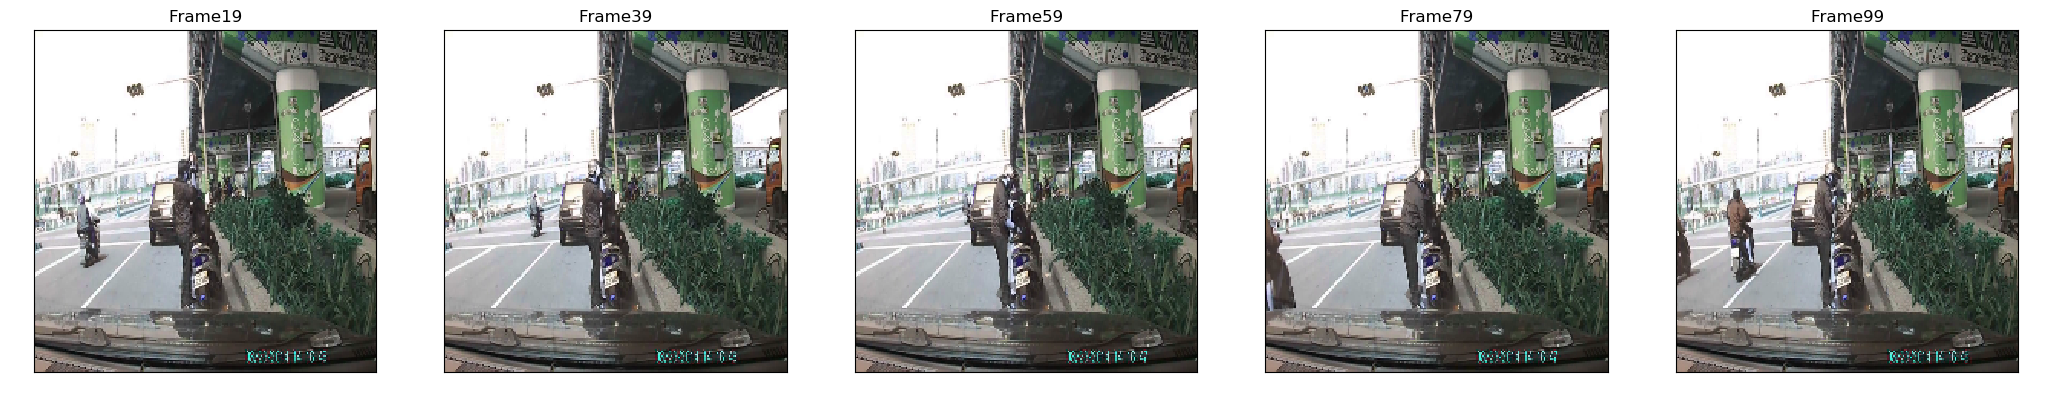
\includegraphics[width=6.5in]{images/level1}
\caption{Low Attention Level Video Sequence}
\label{low}
\end{figure*}

\begin{figure*}[!t]
\centering
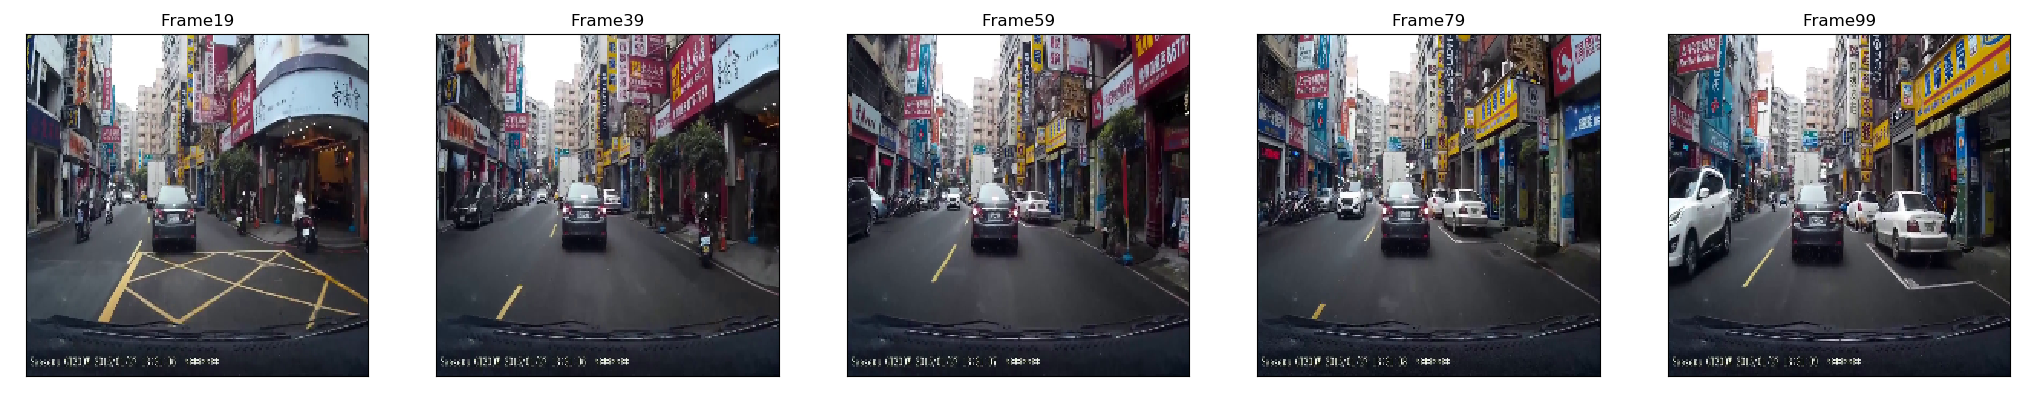
\includegraphics[width=6.5in]{images/level2}
\caption{Medium Attention Level Video Sequence}
\label{med}
\end{figure*}

\begin{figure*}[!t]
\centering
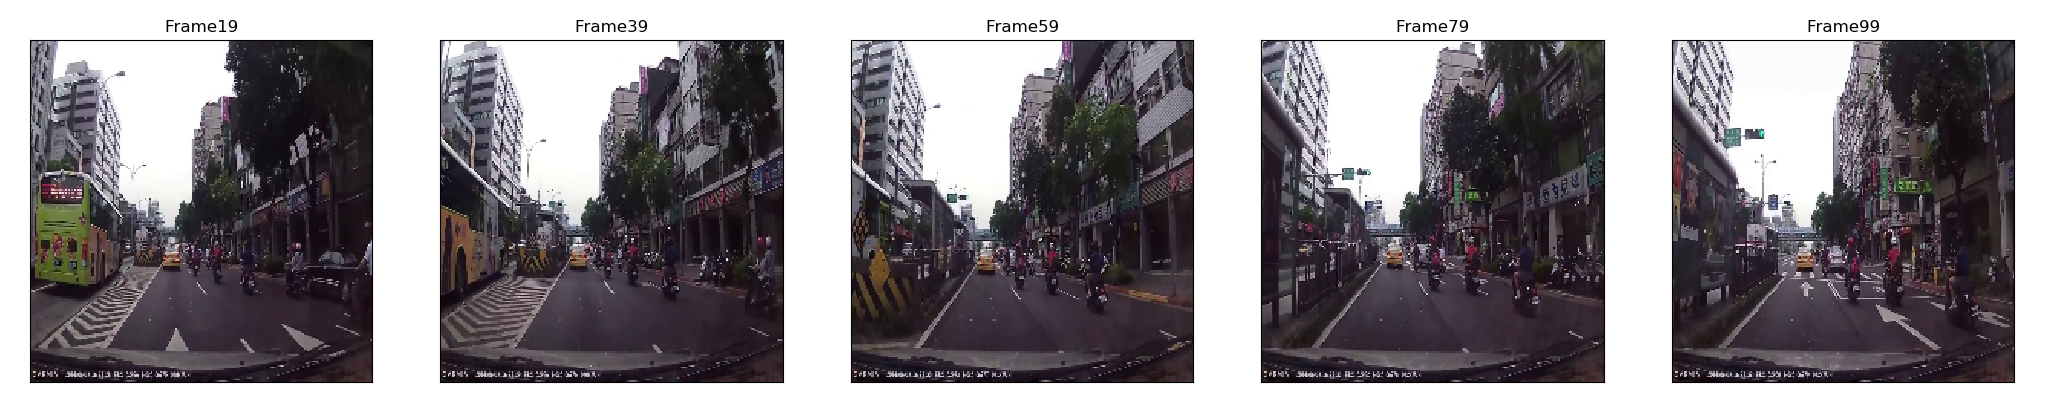
\includegraphics[width=6.5in]{images/level3}
\caption{High Attention Level Video Sequence}
\label{high}
\end{figure*}

\begin{figure*}[!t]
\centering
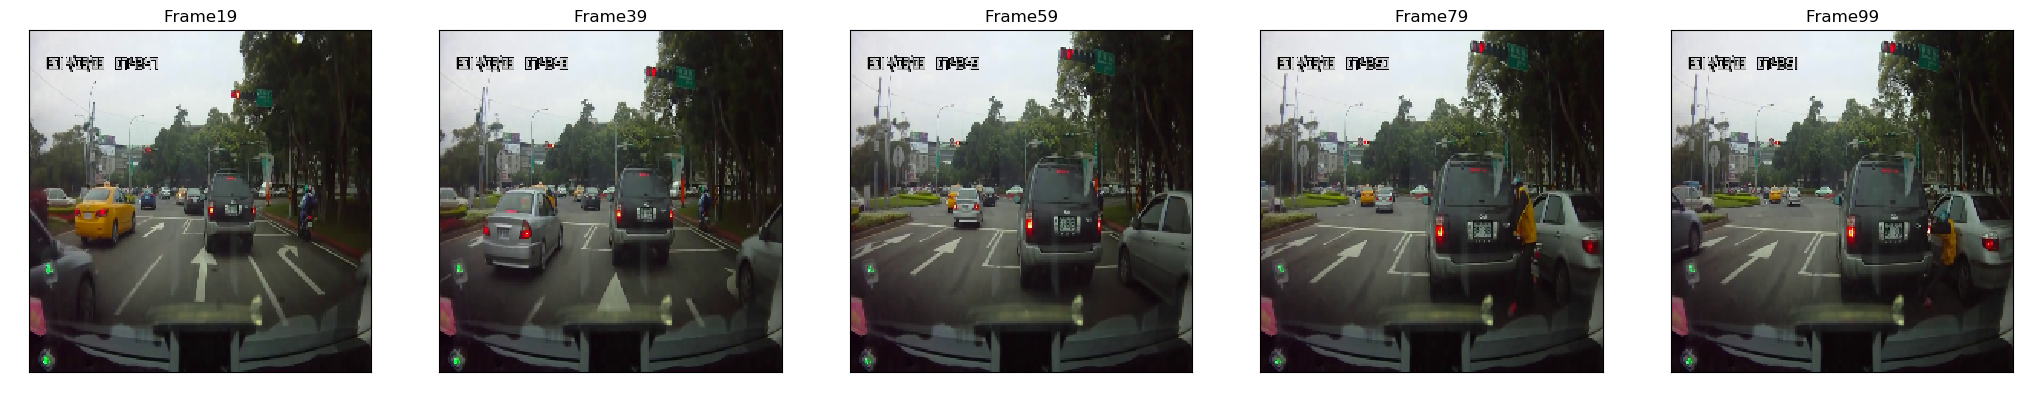
\includegraphics[width=6.5in]{images/level4}
\caption{Very-High Attention Video Sequence}
\label{veryhigh}
\end{figure*}

Initially our approach began by implementing the accident prediction model by Chan et al. \cite{10.1007/978-3-319-54190-7_9}. To differentiate our approach from theirs, we wanted to achieve results in real-time. In order to attain this goal, it was necessary to locate and address the bottleneck in speed. In Chan et al.'s implementation, an advanced feature extraction process was used in which both appearance and motion features are computed. To capture the appearance, a fixed 4096 dimensional feature vector was extracted from each input video frame via a pre-trained VGG network \cite{DBLP:journals/corr/SimonyanZ14a}. For motion features, an improved dense trajectory feature \cite{6751553} for a clip consisting of five consecutive frames was used. PCA helped reduce the dimensionality of trajectory features. Furthermore, a Gaussian-Mixture-Model was trained to produce a clustered feature vector. Lastly, a first-order statistic of fisher vector encoding was used to compute their final feature vector. For our implementation, it was required to remove a lot of this processing time to achieve a real-time implementation. To that end, it was decided to base our full implementation on simple motion estimations based on consecutive frames. The goal here is to see how much information can be gained from flow alone. From here, we wanted to move from the accident prediction problem to attention estimation using the same mindset. To do so, the labeled dataset was created and utilized.

The overall proposed algorithm is broken into three stages: 1) Motion Estimation, 2) Feature Extraction, 3) Attention Labeling. The following sections will describe each of these stages. The complete model is demonstrated in Figure \ref{net}.

\begin{figure}[!t]
\centering
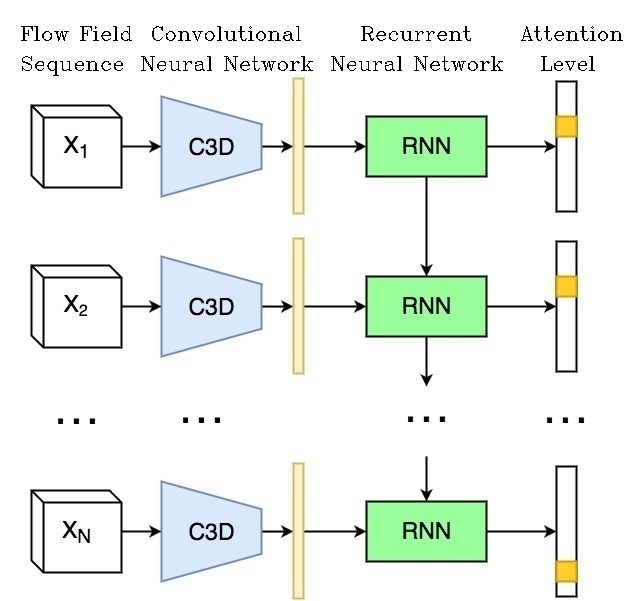
\includegraphics[width=3.5in]{images/net}
\caption{Network Architecture}
\label{net}
\end{figure}

\subsection{Motion Estimation}
The motion estimation used in our proposed algorithm is based on a dense optical flow field. This dense flow field computes optical flow for all points in a pair of frames. An implementation based on Gunner Farneback's algorithm is used \cite{10.1007/3-540-45103-X_50}.

To compute the flow field, a given input video sequence is sampled every five frames and motion estimates are computed between each pair of sampled frames. During training the video sequences are clipped to 100 frames and thus, the resultant flow field sequence length is 19. Additionally, during this stage each frame is resized to a dimensionality of $224 \times 224$. For the computation of optical flow, a window size, pyramid size, and polynomial degree of 15, 3, and 5, respectively, were used. This complete process resulted in a two-channel flow field with flow vectors in the x and y directions. These flow fields were normalized to a range of $[0-1]$. The final output of this stage is a sequence of flow fields with dimensions $19\times 224\times 224\times 2$. Figure \ref{flow} demonstrates an optical flow output.

\begin{figure}[!t]
\centering
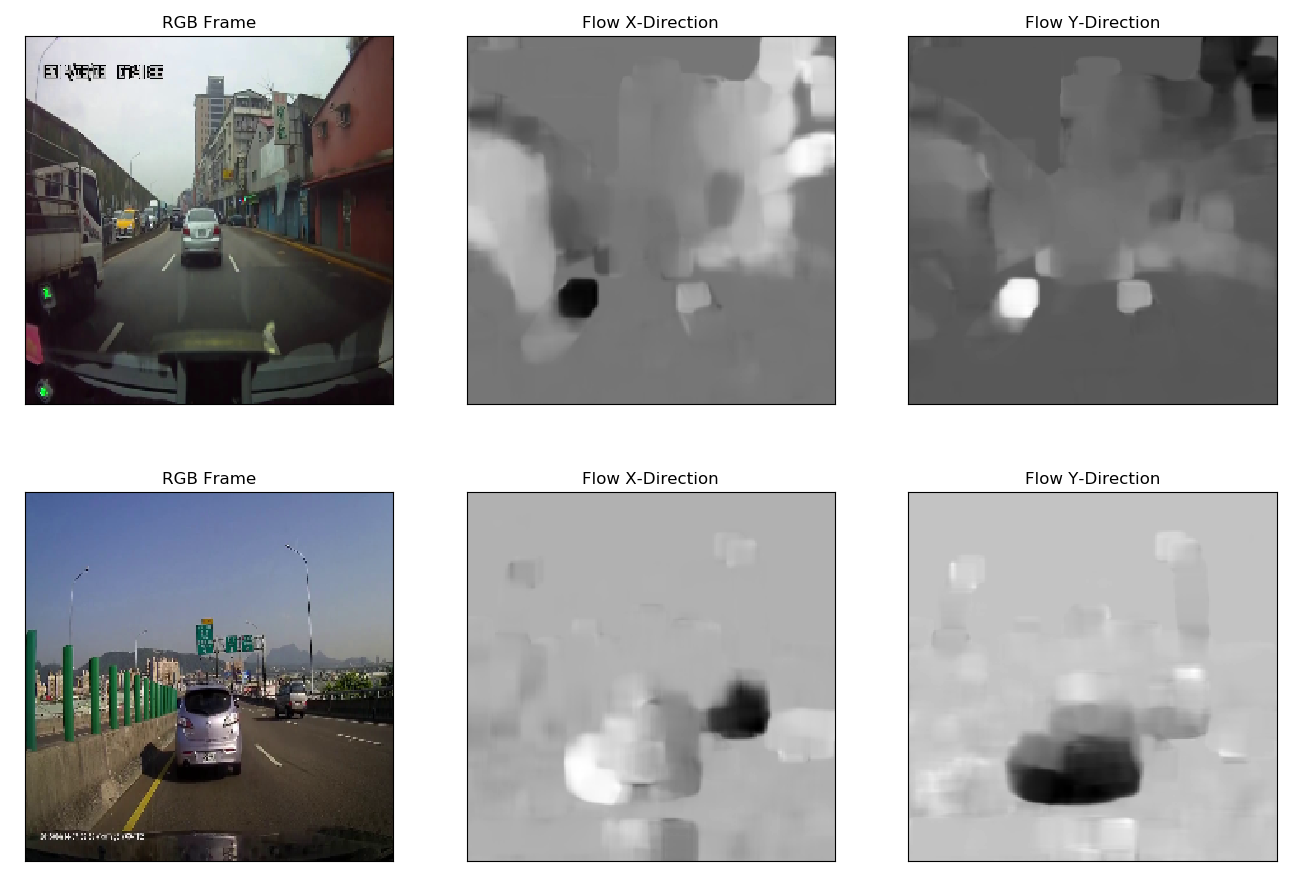
\includegraphics[width=3.5in]{images/flow}
\caption{Optical Flow}
\label{flow}
\end{figure}

\subsection{Convolutional Neural Network}
The second stage of our algorithm is to extract higher-order features from the baseline optical flow features using a convolutional neural network. The CNN model used in our algorithm is a Deep Residual Network \cite{DBLP:journals/corr/HeZRS15}. This ResNet is smaller than some of the newer models as it only consists 18 convolutional and two max-pooling layers. Table 1 summarizes the different layers in this network. Each flow field of dimensionality $224\times224\times2$ is treated as an input image and is passed through the CNN. Through convolution and pooling, the network extracts deep optical flow features that help incorporate additional information than that of the baseline flow fields. To extract these features, the last classification layer of the CNN model is removed, providing a feature dimension of 512. Once all flow sequences are passed through the CNN, the final output dimensionality is $19\times512$. The optical flow CNN features from each frame are then used as input into the next stage.

\begin{table}[!t]
\renewcommand{\arraystretch}{1.3}
\caption{ResNet 18 Model}
\label{resnet18}
\centering
\begin{tabular}{|c|}
\hline
$7 \times 7$, 64, stride 2 \\
\hline
$3 \times 3$ max pool, stride 2\\
\hline
$
\begin{pmatrix}
3 \times 3, 64 \\
3 \times 3, 64
\end{pmatrix}
$
$ \times 2$ \\
\hline
$
\begin{pmatrix}
3 \times 3, 128 \\
3 \times 3, 128
\end{pmatrix}
$
$ \times 2$ \\
\hline
$
\begin{pmatrix}
3 \times 3, 256 \\
3 \times 3, 256
\end{pmatrix}
$
$ \times 2$ \\
\hline
$
\begin{pmatrix}
3 \times 3, 512 \\
3 \times 3, 512
\end{pmatrix}
$
$ \times 2$ \\
\hline
average pool \\
\hline
1000-D FC \\
\hline
\end{tabular}
\end{table}

\subsection{Attention Labeling}
For attention labeling, a recurrent neural network is used. The RNN model used in this paper is a single-layer LSTM network consisting of 128 hidden units. Once all CNN flow features are computed on a given input video, each 512 dimensional feature is passed through the RNN sequentially. The RNN takes as input a given feature vector along with the previous resultant hidden unit. The output of the RNN model is a 128 dimensional feature vector at each time step in the sequence. Since a single attention label is required at the end of the video sequence, only the final 128 dimensional hidden state is passed into the softmax layer. This layer reduces the resulting output size to the required number of labels.

\subsection{Implementation}
The complete attention estimation model is trained via back-propagation using a cross entropy loss function. Adam optimization \cite{DBLP:journals/corr/KingmaB14} was used with a learning rate and batch size of 0.0001 and 50, respectively. Additionally, the CNN-RNN model is trained and tested with PyTorch \cite{paszke2017automatic} on a machine with eight cores, 16GB RAM, and a NVIDIA 970M GPU. The complete model takes approximately ten hours to train.

\section{Experimental Evaluation}
In this section, we report our evaluation results on the driver attention dataset. We use a training, validation, and testing split of 60\%, 20\%, and 20\%, respectively. This split results in 1050 videos used for training and 350 for validation and testing. Figure \ref{plot} demonstrates both the loss function and accuracy plots for both training and validation. As one can see from the graphs, our validation accuracy begins to plateau at approximately 50\%. It is worth noting that the validation loss is lower than the training loss due to dropout layers. These dropout layers are placed between each pair of convolutional layers. The behavior of this layer is different for training and validation cases. During training, a dropout rate of 50\% is used. In the validation phase all features are used, and thus, the validation accuracy is more robust. This situation can lead to lower validation losses and higher validation accuracies, as seen in Figure \ref{plot}. Table 2 displays the best validation score and the associated test score. The final test accuracy received was 50.74\%. Since there are four categories, the complete algorithm produces a score twice that of random chance. The final result demonstrates that estimating the driver's attention level from flow-based processing is a tangible but difficult problem. 

The confusion matrix in Figure \ref{matrix} displays the validation accuracy among various classes. Each row signifies the correct label and each column the predicted label. The algorithm performs best on correctly classifying very high attention levels, however, it sometimes wrongly classifies them to high attention. Additionally, it has trouble classifying high attention situations and generally classifies them to either very high or medium levels.

It is worth noting that one of the features of our proposed system is to provide the driver with an alert when a high or very high attention level is required. To that end, when the overall system produces a false positive it is not necessarily unfavorable as any alert to help focus the driver would be beneficial. Additionally, a false negative is also not necessarily harmful as it produces the same result without driver aid. We believe that any accuracy over random chance provides additional safety to the end user.

Although the flow fields hold some knowledge that relates to the driver's attention level, it may not be enough information to provide a complete understanding of required attention levels. Future iterations of this work would attempt to include more features, namely appearance features, to help improve the accuracy without sacrificing the overall processing speed. 

\begin{figure}[!t]
\centering
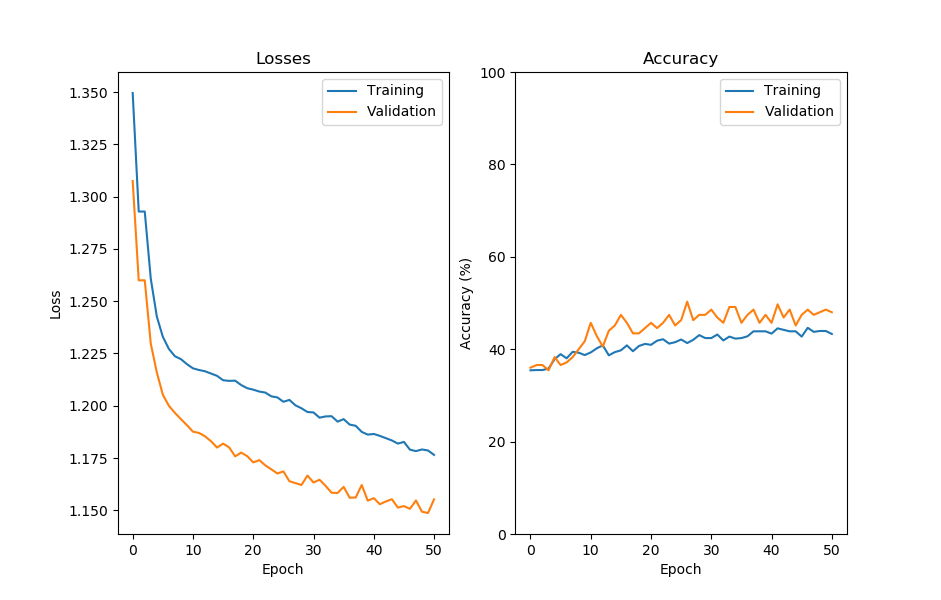
\includegraphics[width=3.5in]{images/plot}
\caption{Training and Validation}
\label{plot}
\end{figure}

\begin{table}[!t]
\renewcommand{\arraystretch}{1.3}
\caption{Model Accuracies}
\label{accuracy}
\centering
\begin{tabular}{|c|c|}
\hline
Validation Accuracy (\%) & Testing Accuracy (\%) \\
\hline
50.29 \% & 50.74 \%\\
\hline
\end{tabular}
\end{table}

\begin{figure}[!t]
\centering
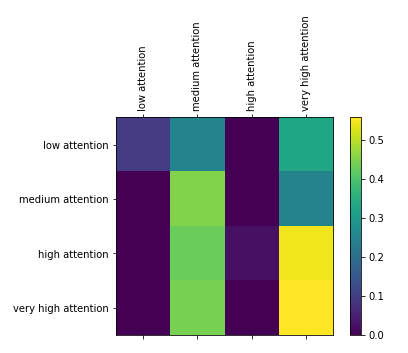
\includegraphics[width=3.5in]{images/matrix}
\caption{Validation Confusion Matrix}
\label{matrix}
\end{figure}

\section{Conclusion}
This paper presented the problem of estimating the driver's perceived attention via dash cam videos. Our proposed approach uses a low-level flow-based method coupled with a convolution and recurrent neural network. We achieve a real-time system that helps alert the driver when a high or very high attention level is required with an accuracy twice that of random change. Our final experimental results demonstrate the effectiveness of using simple flow-based features.
Moving forward, we would like to continue this research to explore how including other fast processing features could help improve the accuracy while still maintaining results in real-time.

\section*{Acknowledgment}
This work is supported by NSERC. Additionally, we gratefully acknowledge Brisk Synergies for providing funding for this research.

\bibliographystyle{IEEEtran}
\bibliography{IEEEabrv,mybib}

\end{document}

